\section{Design}

%This is where the logical / abstract contribution of the project is presented.

%Notice that, when describing a software project, three dimensions need to be taken into account: structure, behaviour, and interaction.

%Always remember to report \textbf{why} a particular design has been chosen.
%Reporting wrong design choices which has been evalued during the design phase is welcome too.

In questa sezione esporremo il design del progetto, partendo dalle decisioni prese in ambito architetturale e proseguendo
col design di dettaglio.

\subsection{Design architetturale}

Come menzionato nei precedenti capitoli, l'obiettivo del progetto è quello di fornire un meccanismo per realizzare sistemi multi-agente distribuiti in \textit{JaKTa}, ed
il gruppo ha deciso di conseguirlo fornendo un' estensione del framework il più minimale possibile.

Dal punto di vista architetturale, il progetto si colloca come modulo aggiuntivo del framework \textit{JaKTa}.

\begin{figure}[h]
    \centering
    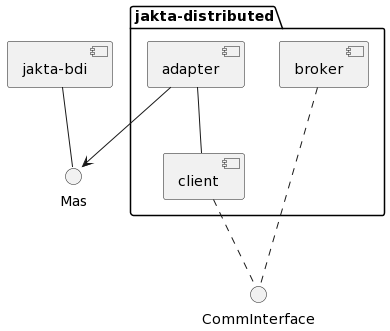
\includegraphics[width=0.8\textwidth]{figures/architecture.png}
    \caption{Architettura del progetto}
    \label{fig:architecture}
\end{figure}

\subsection{Design di dettaglio}
La soluzione proposta consiste nell'implementazione di una versione alternativa dell'interfaccia \textit{Mas}, chiamata \textit{Dmas}, da utilizzare in contesti distribuiti.
Questa estensione dovrà comportarsi come un Mas, ma in aggiunta dovrà essere in grado di comunicare con altri Dmas attraverso la rete utilizzando un protocollo di comunicazione.

Come si può notare dalla figura \ref{fig:architecture}, il progetto è composto da tre componenti principali:

\subsubsection{Adapter}

\subsubsection{Client}

\subsubsection{Broker}


\subsection{Behaviour}

descrizione del main loop del DMas

\subsection{Interaction}

interazione tra vari DMas

interazione tra DMas, client e broker
